\documentclass[a4paper,10pt]{report}
\usepackage[utf8]{inputenc} 
\usepackage{graphicx}
\usepackage[margin=2.5cm]{geometry}
% ---- inclusion de codes
\usepackage{listings} 
\usepackage{color}
\definecolor{lbcolor}{rgb}{0.95,0.95,0.95}
\lstset{frame=single, breaklines=true,showspaces=false,showstringspaces=false,breakautoindent=true, flexiblecolumns=true, keepspaces=true, backgroundcolor=\color{lbcolor}, basicstyle=\ttfamily,basicstyle=\scriptsize, keywordstyle=\color{red}, commentstyle=\color{vert}, stringstyle=\color{blue}, identifierstyle=\ttfamily}

\usepackage[colorlinks=true,linkcolor=black,urlcolor=blue,pdfstartview=FitH]{hyperref} 
\usepackage{float}


% Title Page
\title{High Availability Documentation on OAR - Admin Guide\\

\includegraphics[scale=0.7]{schema/oar_logo_detoure.png}}
\author{Joris Brémond - \texttt{joris.bremond@gmail.com}\\
\\
Laboratoire d'Informatique de Grenoble\\
Bat. ENSIMAG - antenne de Montbonnot\\
ZIRST 51, avenue Jean Kuntzmann\\
38330 MONTBONNOT SAINT MARTIN\\
\\
Authors: LIG laboratory\\
Organization: LIG laboratory\\
Status: Testing\\
Copyright: licenced under the GNU GENERAL PUBLIC LICENSE\\
}




\begin{document}

\maketitle
\tableofcontents

\begin{abstract}
This documentation explain how to configure High Availability on OAR. This solution provide fault tolerance on both OAR server and database (mysql or postgresql).
With this High Availability solution, OAR is protected by computer crash, services crash, network failure, etc.
\end{abstract}












  
\chapter{Introduction}
%schema
\begin{figure}
\begin{center}
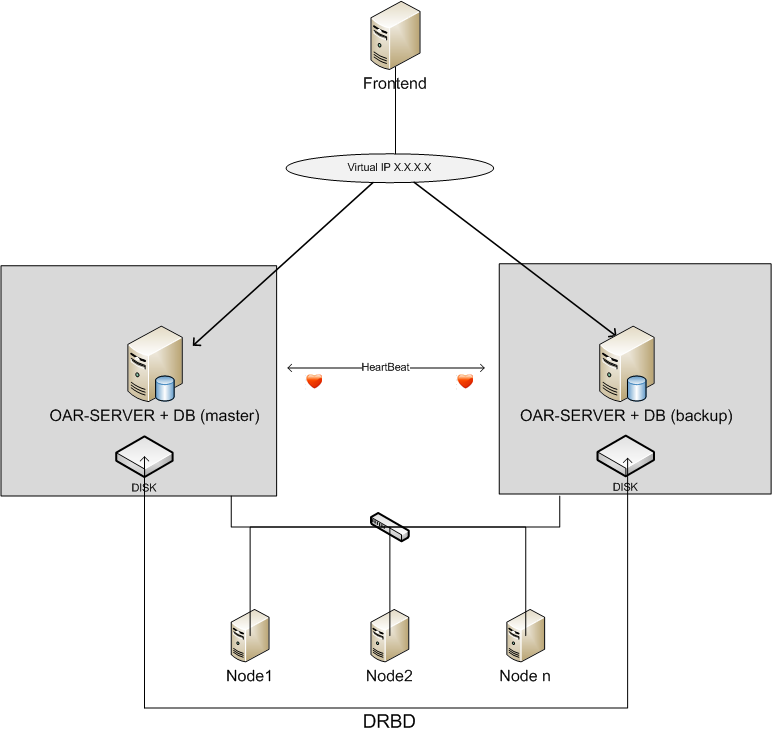
\includegraphics[scale=0.5]{schema/architecture-schema-2-node.png}
\end{center}
\caption{Architecture schema 2 nodes} 
\label{2nodesschema} 
\end{figure} 
\begin{figure}
\begin{center}
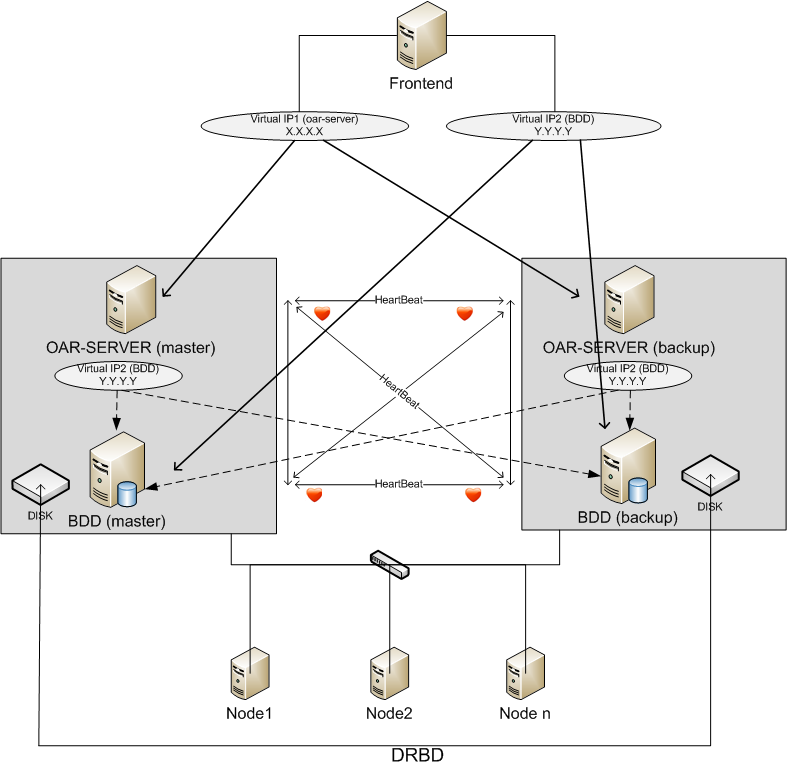
\includegraphics[scale=0.5]{schema/architecture-schema-4-node.png}
\end{center}
\caption{Architecture schema 4 nodes} 
\label{4nodesschema} 
\end{figure} 
\begin{figure}
\begin{center}
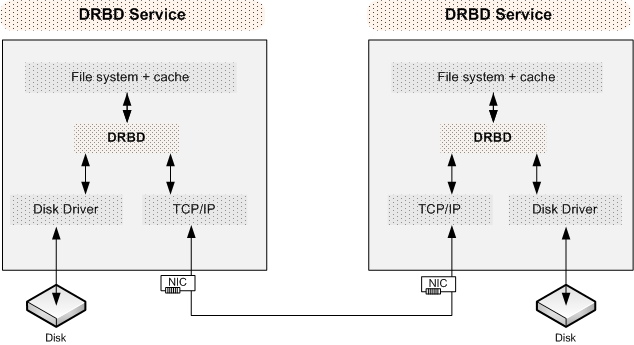
\includegraphics[scale=0.5]{schema/DRBD.png}
\end{center}
\caption{DRBD Architecture} 
\label{drbd} 
\end{figure} 



This documentation explain how to configure a high availability cluster with OAR. We will see two different configurations :
\begin{description}
\item[]- OAR-server daemon and database on the same server. So you have two servers, the master (oar-server + database) and the backup. See Figure \ref{2nodesschema}.


\item[]- OAR-server daemon and database on different server. You have four servers, the master OAR-server, the master database, the backup OAR-server, and the backup database.
See Figure \ref{4nodesschema}.

\end{description}


\section{Require}
This documentation don't describe how to configure and install OAR. So before install OAR High Availability solution, 
install OAR with the database of your choice (mysql or postgresql). OAR-server and database must be also installed on the backup(s) server(s), 
with the same daemon configuration (oar.conf, my.conf or pg.conf). 
Nevertheless, it's not necessary that we configure OAR (oarnodesetting, etc.) because its data are incorporated in database and DRBD will share it. So we will have the same configurations in both nodes.
Before continue, please stop oar-server and database daemon.



\section{General functioning}
For provide OAR High Availability, we use different produces :
\begin{description}
\item[]- The first one is \textbf{Heartbeat} version 2. Heartbeat is a daemon that provides fault tolerance. It manage and monitor services, like Virtual IP, filesystem, etc. When Heartbeat detect problems in resource, it can migrate this one on other server. It can manage groups of resources and define rules and priority on each server.
\item[]- \textbf{DRBD}. DRBD refers to block devices designed as a building block to form high availability clusters. This is done by mirroring a whole block device via an assigned network. DRBD can be understood as network based raid-1. In OAR high availability solution, we will use DRBD for duplicate database.\\
See Figure \ref{drbd}.
\item[]- \textbf{VirtualIP} : This package is installed with heartbeat, and managed by it. It provide a virtual IP address. Thereby, client permanently know the elected server.
When heartbeat active resources on the node, the virtualIP package send a gratuitous ARP. After that, any nodes on the network have in ARP table an entry with :
\begin{lstlisting}
IP address		MAC address primary node
\end{lstlisting}

\end{description}













\chapter{Installation}

Before begin installation on CentOS, verify if the depot "extra" is uncommented, in \textit{/etc/yum.repo.d/CentOS-Base.repo}.
\section{DRBD}
In this guide, we use DRBD-8.
\begin{description}
\item[]- On debian :

The package name is drbd8-utils. It's easier to use module-assistant for install it:
\begin{lstlisting}
apt-get install drbd8-utils module-assistant
module-assistant auto-install drbd8
\end{lstlisting} 



Module Assistant require kernel header. You can install it with :
\begin{lstlisting}
apt-get install linux-headers-`uname -r`
\end{lstlisting}

\item[]- On CentOS :

The package name is drbd82 and kmod-drbd82 for kernel module :
\begin{lstlisting}
yum -y install drbd82 kmod-drbd82
\end{lstlisting} 

\end{description}

Now DRBD is operational.


\section{Heartbeat-2}
Heartbeat has two version. We will use the version 2 because we can monitor each resource and detect service crash.
\begin{description}
\item[]- On debian:

The package name is heartbeat-2.
\begin{lstlisting}
apt-get install heartbeat-2
\end{lstlisting}
You can also install the GUI package on the your computer for heartbeat remote configuration.
\begin{lstlisting}
apt-get install heartbeat-2-gui
\end{lstlisting}

\item[]- On CentOS:

The package name is heartbeat.
\begin{lstlisting}
yum -y install heartbeat
\end{lstlisting}
Verify if heartbeat is completly installed. If not, retry the previous command.

\end{description}











\chapter{Configuration}

For illustrate example, the nodes names are :
\begin{description}
\item[]- 2 nodes configurations : 
\begin{itemize}
\item node1 (master)
\item node2 (backup)
\end{itemize}

\item[]- 4 nodes configurations :
\begin{itemize}
\item node1 (master oar)
\item node2 (master database)
\item node3 (backup oar)
\item node4 (backup database)
\end{itemize}
\end{description}


\section{System configuration}
\label{sysconf}
It's really recommended that we have two different network between each Heartbeat server. Indeed, heartbeat use the network for check its neighbor. With two networks, we can for example avoid split-brain problem (See \ref{splitbrain}). We can use one Ethernet network and one serial network, ore two Ethernet network. With a solution like this, we can easily cut the Ethernet network without interfere with heartbeat functioning.\\

For Heartbeat configuration, we need one or two network address (Virtual IP). If we are in configuration 2 nodes (OAR-server and database on the same nodes), we need one IP address, and two IP if we are in 4 nodes configurations. Two Virtual IP for access to oar-server and database. This virtual IP must be free and accessible on the network.\\

Now, it is heartbeat which launches services like oar, mysql. So you must remove auto launch :
\begin{description}
\item[]- On debian:
\begin{lstlisting}
update-rc.d -f oar-server remove
update-rc.d -f $BD remove
\end{lstlisting}
\item[]- On CentOS:
\begin{lstlisting}
chkconfig oar-server off
chkconfig $BD off
\end{lstlisting}
\end{description}
\$BD correspond to mysql or postgres.\\

DRBD need a low-level storage for write data. It could be an entire disk, a partition, or a virtual partition (in a file). So before configure DRBD, create a free partition.\\
If you want create a partition in a file (/image.img), you can follow this commands :
\begin{lstlisting}
SIZE=200	#Size in Mega-bytes
dd if=/dev/zero of=/image.img bs=1M count=$SIZE
losetup /dev/loop/0 /image.img
mkfs -t ext3 /dev/loop/0
shred -zvf -n 1 /dev/loop/0	
\end{lstlisting}
Furthermore, we need to create a script for auto associate loopback device with the image file at startup, and before DRBD launching.
\begin{description}
\item[]- On debian:
\begin{lstlisting}
#!/bin/sh
case "$1" in
  start|"") 
        losetup /dev/loop0 /image.img
	echo "Start OK"
        ;;
  stop)
	losetup -d /dev/loop0
	echo "Stop OK"
	;;
  *)
        echo "Usage: active-loop [start|stop]" >&2
        exit 3
        ;;
esac
\end{lstlisting}
Change right and add to startup (60 is before DRBD) :
\begin{lstlisting}
chmod +x /etc/init.d/active-loop
update-rc.d active-loop defaults 60
\end{lstlisting}

\item[]- On CentOS:
\begin{lstlisting}
#!/bin/sh
# chkconfig: 2345 60 01
# description: Auto associate loopback with the file image.img
case "$1" in
  start|"") 
        losetup /dev/loop0 /image.img
	echo "Start OK"
        ;;
  stop)
	losetup -d /dev/loop0
	echo "Stop OK"
	;;
  *)
        echo "Usage: active-loop [start|stop]" >&2
        exit 3
        ;;
esac
\end{lstlisting}
Change right and add to startup (60 is before DRBD) :
\begin{lstlisting}
chmod +x /etc/init.d/active-loop
chkconfig --add active-loop
chkconfig --level 2345 active-loop on
\end{lstlisting}
\end{description}

\textbf{Important} : You must verify if the port UDP 694(heartbeat) and TCP 7788(DRBD) is open.

\section{Heartbeat Configuration}

There are three files to configure heartbeat-2 :
\subsection{Authentication file : \textit{/etc/ha.d/authkeys}}
The authkeys configuration file contains informations for Heartbeat to use when authenticating cluster members. It cannot be readable or writable by anyone other than root. For sha authentication, write :
\begin{lstlisting}
auth 1
1 sha1 MyPassword
\end{lstlisting}
You can also use \textbf{md5} or \textbf{crc}.\\
Set file right:
\begin{lstlisting}
chmod 0600 /etc/ha.d/authkeys
\end{lstlisting}

\subsection{Daemon configuration file : \textit{/etc/ha.d/ha.cf}}

The ha.cf file is one of the more important files. It lists the cluster nodes, the communications topology, and which features of the configuration are enabled. 
\begin{itemize}
\item An example with 2 nodes configuration and two Ethernet interfaces :
\begin{lstlisting}
logfile /var/log/ha-log
debugfile /var/log/ha-debug
#use_logd on
udpport 694
keepalive 1 # 1 second
deadtime 10
initdead 80
ucast eth1 IPNODE1
ucast eth1 IPNODE2
ucast eth0_rename IPNODE1
ucast eth0_rename IPNODE2
node node1
node node2
crm yes
\end{lstlisting}

\item For 4 nodes configurations :
\begin{lstlisting}
logfile /var/log/ha-log
debugfile /var/log/ha-debug
#use_logd on
udpport 694
keepalive 1 # 1 second
deadtime 10
initdead 80
ucast eth1 IPNODE1
ucast eth1 IPNODE2
ucast eth1 IPNODE3
ucast eth1 IPNODE4
ucast eth0_rename IPNODE1
ucast eth0_rename IPNODE2
ucast eth0_rename IPNODE3
ucast eth0_rename IPNODE4
node node1
node node2
node node3
node node4
crm yes
\end{lstlisting}
\end{itemize}

\textbf{\underline{details:}}\\
\textbf{keepalive} : x second between each beat\\
\textbf{deadtime} : after x second without heartbeat, the nodes is declared dead\\
\textbf{initdead} : set the time that it takes to declare a cluster node dead when Heartbeat is first started\\
\textbf{ucast}: [interface] [ip node1] network for send/receive heartbeat. You can also use multicast(mcast) or broadcast(bcast) address\\
\textbf{node} : the node names\\
\textbf{crm} : yes for use heartbeat version 2 (very recommended)\\


\subsection{Ressource description file : \textit{/var/lib/heartbeat/crm/cib.xml}}
This file specifies the services manage by heartbeat. We can find three sections :
\begin{itemize}
\item The first one is the cluster property. It describe general cluster behavior. We can specify different options :

\begin{itemize}
\item \textbf{symmetric-cluster} : Is resource can run on any node by default ?
\item \textbf{no-quorum-policy} : Action to do when cluster detect quorum
\item \textbf{default-resource-stickiness} : How much does resource prefer to stay where it is
\item \textbf{default-resource-failure-stickiness} : How many failure before migration
\item \textbf{stonith-enabled} : If true, heartbeat kill the node which have resource failure. You must create a STONITH device before active it.
\item \textbf{stonith-action} : Action to do : reboot or power off
\item \textbf{startup-fencing} : STONITH unseen nodes if true (default)
\item \textbf{stop-orphan-resources} : If true, heartbeat should deleted resource be stopped
\item \textbf{stop-orphan-actions} : If true, should deleted action be canceled
\item \textbf{remove-after-stop} : Remove resources from heartbeat after they are stopped, default = false
\item \textbf{short-resource-names} : true
\item \textbf{transition-idle-timeout} : Provides the default global timeout for actions. Any action which has a defined timeout automatically
uses the action-specific timeout
\item \textbf{default-action-timeout} : How long heartbeat wait for actions to complete
\item \textbf{is-managed-default} : Heartbeat can start or stop resources as required
\item \textbf{cluster-delay} : Round trip delay over the network
\item \textbf{pe-error-series-max} : The number of PE inputs resulting in errors to save. -1 = unlimited
\item \textbf{pe-warn-series-max} : The number of PE inputs resulting in Warnings to save
\item \textbf{pe-input-series-max} : The number of other PE inputs to save
\end{itemize}

\item The second part is the resources properties. We can defined group of resources, and configure them.

\begin{itemize}
\item \textbf{Group definition} : you can create group with the directive :
\begin{lstlisting}[language=xml]
<group id="group1">
\end{lstlisting}
Now, you can add resources in this group.
\item \textbf{Resource definition} : There is two different type of resource : OCF or LSB.\\
OCF example : 
\begin{lstlisting}[language=xml]
<primitive class="ocf" id="resource name" provider="heartbeat" type="resource-name">
\end{lstlisting}
LSB example : 
\begin{lstlisting}[language=xml]
<primitive class="lsb" id="resource name" provider="heartbeat" type="resource-name">
\end{lstlisting}
OCF (Open Cluster Framework) Resource Agents is provided by heartbeat. You can find resource like IPaddr2 (for virtual IP), DRBDdisk for DRBD,etc.
You can also add resource with LSB standard (Linux Standards Base). Generally, it is the main type of resource. The location of the resource you can add is on \textit{/etc/ha.d/resource.d} and \textit{/etc/init.d/}.
When you defined the resource, the type is the name of the resource. Example, if you want to add mysql (/etc/init.d/mysql), you must write : type="mysql". For "id", you can enter the name of your choice.
\item \textbf{Resource operations} : Some operations can be added on resources. In our case, you can add resource monitoring. Example :
\begin{lstlisting}[language=xml]
<operations>
  <op id="VirtualIP-mon" interval="5s" name="monitor" timeout="5s"/>
</operations>
\end{lstlisting}
When the timeout is attained, heartbeat detect resource crash.
\item \textbf{Resources attribute} : Sometimes, resources required additional parameters. You can enter them with the attribute directive :
\begin{lstlisting}[language=xml]
<instance_attributes id="VirtualIP_inst_attr">
  <attributes>
    <nvpair id="VirtualIP_attr_0" name="ip" value="172.16.16.220"/>
    <nvpair id="VirtualIP_attr_1" name="nic" value="eth1"/>
    <nvpair id="VirtualIP_attr_2" name="cidr_netmask" value="24"/>
  </attributes>
</instance_attributes>
\end{lstlisting}

\end{itemize}

\item The last part is resources constraint. You can add constraints on resource or resource group, like location constraint.
In our case, you can specify node priority, for example if you want resources run in priority on master.
\begin{lstlisting}[language=xml]
<constraints>
  <rsc_location id="rsc_location_group_1" rsc="group_1">
    <rule id="prefered_location_group_1" score="100">
      <expression attribute="#uname" id="prefered_location_group_1_expr" operation="eq" value="NODE-NAME"/>
    </rule>
   </rsc_location>
</constraints>
\end{lstlisting}

\item Example of heartbeat configuration cib.xml file : see appendix \ref{cibexample}\\

Tips : The mysql OCF script integrated in heartbeat doesn't work for me, so for avoid to use it, rename the mysql script (just for Debian) in mysqlha for example, and precise it's a LSB script for heartbeat :
\begin{lstlisting}
cp /etc/init.d/mysql /etc/init.d/mysqlha
\end{lstlisting}


\end{itemize}

Now, you must set rights on the cib.xml file, and give it to its owner :
\begin{lstlisting}
chown hacluster:haclient /var/lib/heartbeat/crm/cib.xml
chmod 0600 /var/lib/heartbeat/crm/cib.xml
\end{lstlisting}




\subsection{OAR Service modifications}
\begin{description}
\item[]- On debian:\\

The OAR service (/etc/init.d/oar-server) is currently not compatible with LSB standard. It haven't the status function. So heartbeat can't monitor it.
For add status function on oar-server, edit \textit{/etc/init.d/oar-server} file, and add :
\begin{lstlisting}[language=bash]
status)
	if [ -f $PIDFILE ]
	then
		PID=`head -n 1 $PIDFILE`
		if [ `ps -ef | grep -v grep | grep $PID | wc -l` -ge 1 ]
		then
			echo "OAR is running"
			exit 0
		else
			echo "OAR is not runnig"
			exit 2
		fi
	else
		echo "OAR is not runnig"
		exit 2
	fi
	;;
\end{lstlisting}

\item[]- On CentOS:\\

The return value in CentOS is different that Debian. For example, if you stop oar-server which runs, and action success, oar service return 0. But if it is already stopped, Debian return 0 but not CentOS. So heartbeat failed in monitor mode, because if don't have the right return value.
You must modify the "stop" option :
\begin{lstlisting}[language=bash]
stop() {
        echo -n "Stopping $DESC: "
        if [ -n "`pidfileofproc $DAEMON`" ]; then
            killproc $DAEMON
            sleep 1
            killall Almighty 2>/dev/null
            sleep 1
            killall -9 Almighty 2>/dev/null
            RETVAL=0
        else
            failure $"Stopping $DESC"
            RETVAL=$?
            if [ `ps -ef | grep -v "grep" | grep Almighty | wc -l` -eq 0 ]; then
                RETVAL=0
            fi
        fi
        echo 
}
\end{lstlisting}
\end{description}

\section{DRBD Configuration}
In DRBD configuration file, we can specifies a lots of parameters, which describe resources, synchronization type, synchronization rate, etc. For a complete example, see \ref{drbdexample}.
\subsection{synchronization type}
DRBD has three synchronization type :
\begin{itemize}
\item \textbf{Protocol A} : write ACK (on master) is send when data was transmitted on master disk and sent to slave.
\item \textbf{Protocol B} : write ACK (on master) is send when data was transmitted on master disk and received by slave.
\item \textbf{Protocol C} : write ACK (on master) is send when data was transmitted on master disk and slave disk.\\
\textbf{Very recommended !}
\end{itemize}

\subsection{Startup action}
When DRBD is launched, we can do actions. For example, inform it to wait x seconds :
\begin{lstlisting}
startup {
  wfc-timeout x;
}
\end{lstlisting}

\subsection{Disk action}
The directive ``disk'' can add action to do for disk. It's recommended to add this one :
\begin{lstlisting}
disk {
  on-io-error detach;
}
\end{lstlisting}
With the detach option, the node drops its backing device on I/O error, and continues in diskless mode.

\subsection{Synchronization settings}
You can precise the rate of synchronization, the hot-area size :
\begin{lstlisting}
syncer {
  rate 700000K;
  al-extents 257;
}
\end{lstlisting}
700000K is the maximum value accepted by DRBD.\\
al-extend corresponds to 4 Mbytes, so with 257, we have 1 GBytes.

\subsection{Host section}
\label{hostsection} 
One resource must have two host section. A host section describe on each node which DRBD partition and disk is used. You must also specify neighbor ip and port :
\begin{lstlisting}
resource mysql {
  on node1 {
    device DRBDPARTITION;
    disk DISKPARTITION;
    address node2:DBRDPORT;
    meta-disk internal;
  }

  on node2 {
    device DRBDPARTITION;
    disk DISKPARTITION;
    address node1:DBRDPORT;
    meta-disk internal;
  }
}
\end{lstlisting}

\subsection{Handlers}
DRBD provide an handler which can execute actions on events. For the problem of split brain (see \ref{splitbrain}), you can for example write in log :
\begin{lstlisting}
handlers {
  split-brain "echo Splitbraindetected >> /var/log/drbd-log"
  pri-lost-after-sb "echo pri-lost-after-sb >> /var/log/drbd-log"
}

net {
  #cram-hmac-alg \"sha1\";
  #shared-secret \"123456\";
  after-sb-0pri discard-younger-primary;
  after-sb-1pri consensus;
  after-sb-2pri call-pri-lost-after-sb;
  #rr-conflict violently;
}
\end{lstlisting}
In the net directive, you can specifies different policies when you detect split brain.\\
\textbf{after-sb-0pri} : Split brain has just been detected, but at this time the resource is not in the Primary role on any host.
\begin{itemize}
\item disconnect : Do not recover automatically, call split-brain handler script, drop the connection and continue in disconnected mode.
\item discard-younger-primary : Discard and roll back the modifications made on the host which assumed the Primary role last.
\item discard-least-changes : Discard and roll back the modifications on the host where fewer changes occurred.
\item discard-zero-changes : If there is any host on which no changes occurred at all, simply apply all modifications made on the other and continue.
\end{itemize}
\textbf{after-sb-1pri} : Split brain has just been detected, and at this time the resource is in the Primary role on one host.
\begin{itemize}
\item disconnect 
\item consensus : Apply the same recovery policies as specified in after-sb-0pri. If a split brain victim can be selected after applying these policies, automatically resolve. Otherwise, behave exactly as if disconnect were specified.
\item call-pri-lost-after-sb : Apply the recovery policies as specified in after-sb-0pri. If a split brain victim can be selected after applying these policies, invoke the pri-lost-after-sb handler on the victim node.
\item discard-secondary : Whichever host is currently in the Secondary role, make that host the split brain victim.
\end{itemize}
\textbf{after-sb-2pri} : Split brain has just been detected, and at this time the resource is in the Primary role on both hosts. This option accepts the same keywords as after-sb-1pri except discard-secondary and consensus.

\subsection{Launch DRBD}
Before launch DRBD between the two host, you can prepare the device. The first things to do, is to load DRBD module :
\begin{lstlisting}
 modprobe drbd
\end{lstlisting}
After that, you must verify if the drbd device exist. Look at /dev/drbd0. If this device don't exist, create it with :
\begin{lstlisting}
mknod /dev/drbd0 b 147 0
\end{lstlisting}
Now, it is the time to create meta data and launch DRBD :
\begin{lstlisting}
drbdadm create-md all
drbdadm up all
\end{lstlisting}
For mount DRBD device, you must create a folder, /mnt/drbdata for example :
\begin{lstlisting}
mkdir /mnt/drbddata
\end{lstlisting}
DRBD is practically operational. You have to defined a master, node1 in our example, so enter this command only on this node :
\begin{lstlisting}
drbdadm -- --overwrite-data-of-peer primary all

mkfs -t ext3 /dev/drbd0
mount /dev/drbd0 /dev/drbddata
\end{lstlisting}
The ``all'' option mean that node1 is the master of all resources defined in drbd.conf.\\
The mkfs command prepare file system on drbd partition, and mount this partition.\\
Now DRBD is operational, all data put in \textbf{/dev/drbddata} will be synchronized.




\section{Database Configuration}
Now, it is the time to configure database. The datadir will be changed into the  mount point of disk partition defined in DRBD (see  \ref{hostsection}).

\subsection{Mysql}
For change datadir in mysql, open the file \textit{/etc/mysql/my.cnf} for Debian or \textit{/etc/my.cnf} for CentOS, search the primitive \textbf{datadir}, and replace the value by the partition defined in DRBD.
For example, we can enter :
\begin{lstlisting}
datadir = /mnt/drbddata
\end{lstlisting}
You must copy all old mysql data in new datadir, and change owner :
\begin{lstlisting}
cp -r /var/lib/mysql /mnt/drbddata
chown -R mysql:mysql /mnt/drbddata/mysql
\end{lstlisting}
If you want remote mysql access, don't forget to comment the \textbf{bind-address} in the my.cnf.\\

In CentOS, you must correct a problem, like for oar-server, with the return value. At the begining of the "stop" option in \textit{/etc/init.d/mysqld}, add :
\begin{lstlisting}
stop(){
  status mysqld
  if [ $? -eq 3 ]; then
      action $"Stopping $prog: " /bin/true
      exit 0
  fi
  ...
\end{lstlisting}

\subsection{Postgresql}
It is almost the same in Postgres. Open the file \textit{/etc/postgres/'version'/main/postgresql.conf}, and search data\_directory and change value in :
\begin{lstlisting}
data_directory = 'mnt/drbddata/main'
\end{lstlisting}
Like mysql, if you want remote access, change \textbf{listen\_addresses = 'localhost'} in \textbf{listen\_addresses = '*'}. Don't forget to add rule for your network in the hba.conf file.\\
You must copy all old postgres data in new datadir, and change owner :
\begin{lstlisting}
cp -r /var/lib/postgresql/'version'/main /mnt/drbddata
chown -R postgres:postgres /mnt/drbddata/main
\end{lstlisting}



\section{OAR Configuration}
\subsection{Server configuration}
OAR server must be configured to work fine with High Availability. The first step is to configure database hostname and server hostname on oar-server.
\begin{itemize}
 \item In 2 nodes configurations, one virtual IP is necessary. With this IP, client can access to oar-server and database because it is on the same server.
So in \textit{/etc/oar/oar.conf}, modify :
\begin{lstlisting}
SERVER_HOSTNAME=VIRTUALIP
DB_HOSTNAME=VIRTUALIP
\end{lstlisting}
\item In 4 nodes configurations, two virtual IP is necessary. The first one is for oar-server, and the second is for database.
So in \textit{/etc/oar/oar.conf}, modify :
\begin{lstlisting}
SERVER_HOSTNAME=VIRTUALIP_1
DB_HOSTNAME=VIRTUALIP_2
\end{lstlisting}

\end{itemize}


The second step is to configure the \textbf{DETACH\_JOB\_FROM\_SERVER} option. Indeed, with this option, oar don't keep connection between oar-server and nodes.
So when the oar-server crash, the backup oar-server is contacted when the job is ended, because oarexec reconnect to the new server, thanks to VIRTUALIP\_1.\\
In /etc/oar/oar.conf, you must enter :
\begin{lstlisting}
DETACH_JOB_FROM_SERVER="1"
\end{lstlisting}

\textbf{insert schema !!!}

\subsection{Frontend configuration}
\label{frontendconf}
It is approximately the same configuration on frontend :\\
\begin{itemize}
 \item In 2 nodes configurations :
\begin{lstlisting}
SERVER_HOSTNAME=VIRTUALIP
DB_HOSTNAME=VIRTUALIP
\end{lstlisting}
\item In 4 nodes configurations :
\begin{lstlisting}
SERVER_HOSTNAME=VIRTUALIP_1
DB_HOSTNAME=VIRTUALIP_2
\end{lstlisting}
\end{itemize}

\subsection{Node configuration}
\label{nodeconf}
If you use Start/Stop of nodes using ssh keys (see http://wiki-oar.imag.fr/index.php/Configuration\_tips section 1.5) and you want to do oarnodesetting form oar-server, 
you have just to add the virtual IP from OAR-server in \textit{/etc/default/oar-nodes} file.
\begin{lstlisting}
OARREMOTE=VIRTUALIP
\end{lstlisting}

\section{Administration commands}

\subsection{Heartbeat administration}

Before read more, heartbeat and drbd must be configured and started. For launch heartbeat, run :
\begin{lstlisting}
/etc/init.d/heartbeat start
\end{lstlisting}


\subsubsection{Heartbeat-gui}

\begin{figure}
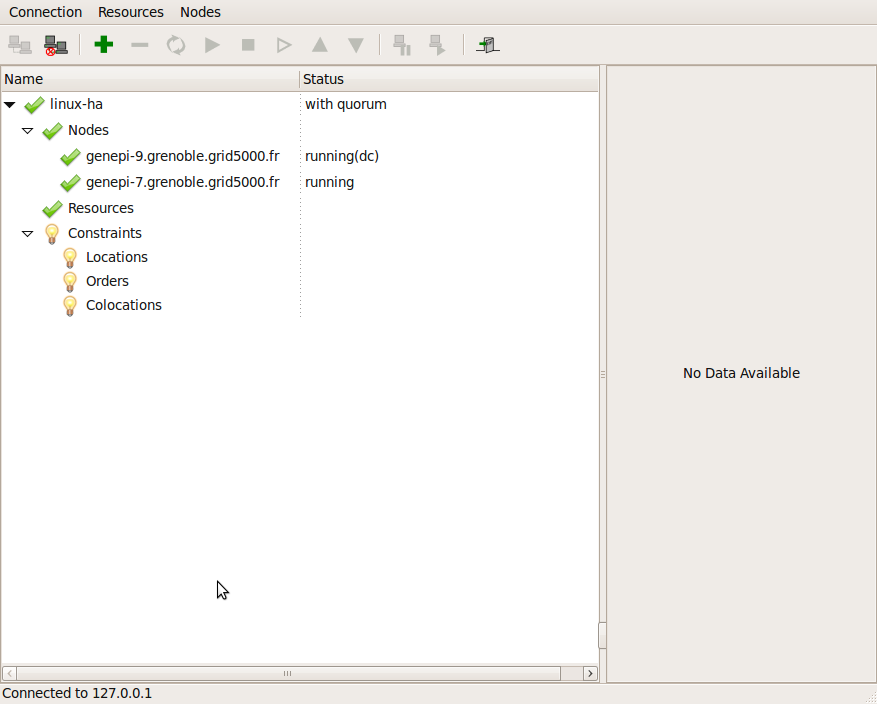
\includegraphics[scale=0.5]{schema/hb_gui-2nodes-connect.png}
\caption{heartbeat-gui connection} 
\label{hb-gui-connect} 
\end{figure}

\begin{figure}
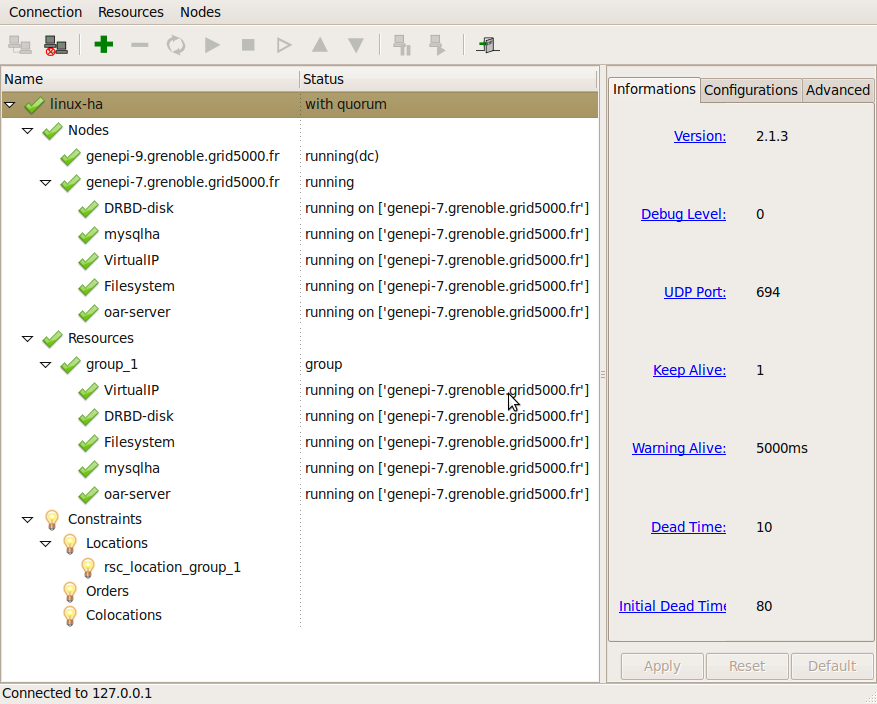
\includegraphics[scale=0.5]{schema/hb_gui-2nodes.png}
\caption{heartbeat-gui 2 nodes example} 
\label{hb-gui-2nodes} 
\end{figure}


Heartbeat provide a graphic interface for configure resources. You can install the package heartbeat2-gui on a remote computer, with the command(on debian) :
\begin{lstlisting}
apt-get install heartbeat2-gui
\end{lstlisting}
on CentOS :
\begin{lstlisting}
yum install heartbeat-gui
\end{lstlisting}
If you work on grid5000, you must create a ssh tunnel on port 5560. Example :
\begin{lstlisting}
ssh -L 5560:machine.grid5000.fr:5560 login@access.site.grid5000.fr
\end{lstlisting}
When you launch heartbeat-gui, it demands login and password. On the heartbeat server, defined a new password for \textbf{hacluster} user :
\begin{lstlisting}
passwd hacluster
\end{lstlisting}
Now you can connect with user hacluster and his password.\\

When you are connected, you can see your configured nodes, and resources if you defined them in the cib.xml file. The figure \ref{hb-gui-connect} show a heartbeat cluster without resources.\\

For add resource, right click on \textbf{Resources}, and choose \textbf{Add New Item}, \textbf{Native}. Now select the resource, add parameter if you want, and click \textbf{Add}.\\
You can add group with the same operations, but select \textbf{Group} in place of \textbf{Native}. Select \textbf{Ordered} for launched resources with order.\\

It is also possible to add location constraint with heartbeat-gui. Select \textbf{Location}, and the group or resource for apply this constraint.\\

For launched resources, click right on the resource, and select \textbf{start}.\\

If a resource failed to start for example, you must cleanup the resource. You can do this by right click on the resource, and select \textbf{Cleanup resource}.\\

For test your configurations, you can standby one node, and see if resource migrate. For Standby a node, right click on it and select \textbf{Standby}.

The figure \ref{hb-gui-2nodes} is an example with 2 nodes configurations and mysql.

\subsubsection{Heartbeat command-line}
\label{hb-command}
Different commands are available : 
\begin{enumerate}
 \item crmadmin - provide node related details 
 \item cibadmin - allows the current configuration to be queried and modified \\
    You can change the cib.xml file with these commands :
    \begin{lstlisting}
    cibadmin -Q > cibbackup.xml 
    \end{lstlisting}
  Apply change on cibbackup.xml and apply it with :
    \begin{lstlisting}
    cibadmin -R -x cibbackup.xml 
    \end{lstlisting}

 \item crm\_verify - checks if configuration is valid 
 \item crm\_mon - provides the current cluster status in text or HTML , see \ref{hb-monitor}
 \item crm\_resource - query and modify all things related to cluster resources/services\\
    Scenario : The resources OAR is crashed and don't restart. Heartbeat migrate on the second node. When you have corrected the problem on the first node, you must cleanup the resource with the command :
    \begin{lstlisting}
    crm_resource -C -r oar-server -H host
    \end{lstlisting}
 \item crm\_standby - control a node's standby status (ability to run resources) \\
    Set node in standby mode :
    \begin{lstlisting}
    crm_standby -U host -v true 
    \end{lstlisting}
 \item cl\_status - provides low-level node-centric connectivity information. 
\end{enumerate}



\subsection{DRBD administration}
\label{drbd-admn}
\begin{itemize}
 \item attach and connect all DRBD resources :
    \begin{lstlisting}
    drbdadm up all
    \end{lstlisting}
\item detach and disconnect all DRBD resources :
    \begin{lstlisting}
    drbdadm down all
    \end{lstlisting}

\item Put node in primary mode :
    \begin{lstlisting}
    drbdadm primary all
    \end{lstlisting}

\item Put node in secondary mode :
    \begin{lstlisting}
    drbdadm secondary all
    \end{lstlisting}

\item After a slipt-brain (see \ref{splitbrain}), you must invalidate data on one node, and reconnect it. The command \textit{cat /proc/drbd} indicates standalone mode.
    \begin{lstlisting}
    drbdadm invalidate all
    drbdadm connect all
    \end{lstlisting}

\end{itemize}




\section{Monitoring utils}

\subsection{Heartbeat monitoring}
\label{hb-monitor}
Heartbeat-2 provide different solutions for monitor resources and know nodes status.
\begin{itemize}
 \item Command line solution : On any heartbeat nodes, you can enter :
\begin{lstlisting}
crm_mon -i 1
\end{lstlisting}
You can see nodes status, and where resources are launched, follow failed actions.
\item Web solution : you can monitor resource with a cgi script. For install it, create a file in \textbf{cgi-bin} path, \textit{/usr/lib/cgi-bin/ha-status.cgi} on Debian or \textit{/var/www/cgi-bin/ha-status.cgi} on CentOS:
\begin{lstlisting}
#!/bin/bash
sudo /usr/sbin/crm_mon -w
\end{lstlisting}
Add apache (www-data) in the sudoers file (for Debian) :
\begin{lstlisting}
echo 'www-data ALL=NOPASSWD:/usr/sbin/crm_mon' >> /etc/sudoers
\end{lstlisting}
For CentOS, add the user apache in the sudoers file and comment the line  \textit{Defaults  requiretty} for enable sudo in tty mode:
\begin{lstlisting}
echo 'apache ALL=NOPASSWD:/usr/sbin/crm_mon' >> /etc/sudoers
\end{lstlisting}
Set right :
\begin{lstlisting}
chmod 755 .../ha-status.cgi
\end{lstlisting}
Now you can access to heartbeat status with http://x.x.x.x/cgi-bin/ha-status.cgi
\item Logs : you can access to heartbeat log in \textit{/var/log/ha-log}

\end{itemize}


\subsection{DRBD monitoring}
For know DRBD status, you can type :\\
\begin{lstlisting}
cat /proc/drbd
\end{lstlisting}


You can know who is the primary/secondary, if DRBD is connected, uptodate, have detect split-brain. If you have a running configuration, you may have :
\begin{figure}[!h]
\begin{center}
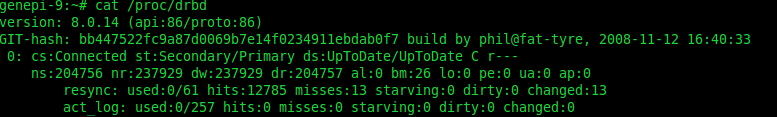
\includegraphics[scale=0.5]{schema/drbd-s-p.png}
\end{center}
\caption{DRBD secondary primary} 
\label{hb-gui-2nodes} 
\end{figure}

\chapter{known problems}
\section{Quorum}
The quorum calculation process is required to select no more than one primary subcluster at a time. You can enable or disable this option in heartbeat, it depend to the configuration.\\
A common method for defining quorum is to say that a subcluster of size n in a cluster of m total nodes has quorum if it has a plurality of nodes in its partition. That is, it has n members where n \textgreater INT(m/2).\\
But this solution in heartbeat create problems in 4 nodes configurations. Indeed, when 2 nodes are down, the two other not can't launch resources because they haven't quorum. In this case, you
can disable quorum in heartbeat, in the cib.xml file :
\begin{lstlisting}[language=xml]
<nvpair id="cib-bootstrap-options-no-quorum-policy" name="no-quorum-policy" value="ignore"/>
\end{lstlisting}


\section{Split brain}
\label{splitbrain} 
When a cluster thinks the other is unavailable, and vice versa, heartbeat launches resources on two nodes. In our configurations, DRBD becomes primary on two nodes, and has two version of data. This problem may appear when the communication between the two heartbeat server is loosed.
For limit this problem, you can connect two links between each heartbeat server.



\section{File System Check}
A fail over must be fastest as possible. So it could be very embarrassing if we have a file system check during the fail-over. You can deactivate it with :
\begin{lstlisting}
tune2fs -c 0 DISKPARTITION
\end{lstlisting}

\chapter{High Availability auto installation}

You can install High Availability on OAR with HAinstal bash script. This script must be launched on each node you want to make faul tolerant, with root rights. Example, 2 nodes for oar-server and database on the same server (the master with oar-server and database, and the backup), and 4 nodes (master oar-server, master database, backup oar-server, backup database) if it different.
Like previously, you must have a working installation (oar, database) : oar must access to database, etc.. This script don't configure frontend and nodes, so you must to refer to \ref{frontendconf} and \ref{nodeconf}.

\section{Prerequisites}
\begin{itemize}
 \item Root rights
 \item Oar and database already installed and ready to work (without High availability)
 \item Linux-hearders (only on Debian): 
    \begin{lstlisting}
    apt-get install linux-headers-`uname -r`
    \end{lstlisting}
 \item For CentOS : access to the depot "extra"
 \item One or two free IP address (for virtual IP)
 \item A free partition, or selected option USEFILEPARTITION
\end{itemize}


\section{Parameters}

\begin{itemize}
 \item Package name :\\
    \begin{lstlisting}
    DRBD="drbd8-utils"
    HEARTBEAT2="heartbeat-2"
    MODULEASSITANT="module-assistant"
    \end{lstlisting}
  This variable contains debian package name of DRBD, heartbeat-2, and module assistant. MODULEASSISTANT is only used on the Debian script.

 \item BDD :\\
  \begin{lstlisting}
  # "mysql" or "postgresql"
  BD="postgresql" or BD="mysql"
  ##only for postgres
  PGVERSION="8.3"
  \end{lstlisting}
The BD variable must be mysql or postgresql. If we choose postgresql, you must enter the version, for script access into service directory, like \textit{/etc/postgresql/8.3/main/postgresql.conf}.

 \item Nodes name :\\
  \begin{lstlisting}
  MASTER_OAR="genepi-7.grenoble.grid5000.fr"
  MASTER_DB="genepi-7.grenoble.grid5000.fr"
  BACKUP_OAR="genepi-9.grenoble.grid5000.fr"
  BACKUP_DB="genepi-9.grenoble.grid5000.fr"
  \end{lstlisting}
The name must be the result of \textbf{uname -n} command, for each node.

  \item Nodes properties :\\
  \begin{lstlisting}
  #Interface
  ETH="eth1"
  #OAR-server Virtual IP (ex : )
  IP="172.16.16.220"
  #Database Virtual IP (ex : 172.16.16.221)
  IP_DB="172.16.16.221"
  #enter CIDR netmask (ex : 24)
  MASK="24"
  \end{lstlisting}
The ETH variable is the network interface uses for heartbeat. IP and IP\_DB are the two virtual IP. If you are in 2 nodes configurations, IP\_DB is ignored.

  \item Heartbeat configuration :\\
  \begin{lstlisting}
  ##Password sha
  PASSWORD="oarteam"
  ##UDP Port
  HBPORT="694"
  \end{lstlisting}
The password is used for heartbeat connection. The default heartbeat port is UDP 694.

 \item DRBD configuration
\begin{enumerate}
 \item PARTITION :\\
  \begin{lstlisting}
    #--low-level storage for the drbd data (partition)---#
    #It could be a loopback device, like /dev/loop0
    DISKPARTITION=/dev/loop0

    #Do you want create a partition in a file ?  ("y" or "n") --> The DISKPARTTION Must be a loopback interface
    USEFILEPARTITION="y"
  \end{lstlisting}
If you want use partition in a file (like describe in \ref{sysconf}), write "y". If you have choose "y" :
  \begin{lstlisting}
    #-PATH File image-#
    IMAGE=/image.img
    #Size in MegaBytes
    SIZE="200"
  \end{lstlisting}
  
  \item DRBD device :\\
  \begin{lstlisting}
    #----DRBD partition alias---#
    DRBDPARTITION=/dev/drbd0

    #----DRBD mount point---#
    DRBDDATA=/mnt/drbddata

    #---FileSystem type (ext2,ext3)---#
    FSTYPE="ext3"
  \end{lstlisting}
The mount point is where you want mount shared data with DRBD.

  \item DRBD port :\\
  \begin{lstlisting}
    ##DRBD communication Port
    DBRDPORT="7788"
  \end{lstlisting}
  
\end{enumerate}

\item CGI script :\\
  If you want to use CGI script for monitor heartbeat, say "y", else "n"
  \begin{lstlisting}
    CGI="y"
  \end{lstlisting}

\end{itemize}



\section{How does it work}
\begin{itemize}
 \item Initialization: \\
Thanks to "uname -n" command, script checks if you are in 2 nodes configurations or not, if the node is the master, backup, etc.
 \item Functions:\\
This part contains useful function. The function exists is used for verify if any commands used by the script is present. For example, the script tests if the command "losetup" is available.
 \item Prerequisites test:\\
Test with the function exists, view above.
 \item Installation:\\
The installation part installs heartbeat version 2 and DRBD 8 if the node must run database.
 \item Stop service:\\
Before modify service configuration, it is recommended to stop it.
 \item Heartbeat configuration:\\
In this part the script configures heartbeat. It copies configurations in three files : \textit{/etc/ha.d/authkeys}, \textit{/etc/ha.d/ha.cf}, \textit{/var/lib/heartbeat/crm/cib.xml}. The configuration is different if you are in 2 or 4 nodes configuration. So the script contains different scenario.
 \item OAR service modification:\\
There are different modifications to do for OAR service. For Debian, the init script don't have the status function. For CentOS, the script must change the return value for better heartbeat compatibility.
 \item OAR configuration:\\
Now, the script configures OAR with the detach mode, put the virtual IP address for database and par-server hostname.
 \item Database configuration:\\
For database, the script defines the data directory.
 \item DRBD configuration:\\
Copy DRBD configuration file \textit{/etc/drbd.conf}. After that, it loads drbd module, creates the image file if you have set USEFILEPARTITION to "y", copies old mysql data into the DRBD device, and puts the two nodes in secondary mode.
 \item Remove auto-launch services:\\
After installation, only heartbeat must manage services like oar-server, database, etc. So the system mustn't start services automatically.
 \item Automatic association of loopback device with image:\\
If you have set USEFILEPARTITION to "y", the system must associate the file image.img to the loopback interface, before DRBD start. So the script creates a startup script which realizes this action automatically.
 \item Add cgi script:\\
If you want monitor heartbeat over HTTP, the script creates a CGI script, accessible via http//x.x.x.x/cgi-bin/ha-status.cgi
\end{itemize}





\chapter{Test}

\section{DRBD performance test}

For know DRBD performance, I have realized different benchmark with mysql for test DRBD performance. This test uses DRBD in synchronous mode (protocol C in drbd.conf).\\
\textbf{Test environments :}
\begin{enumerate}
 \item Master DRBD was genepi-31.grenoble.grid5000.fr. The test without DRBD was also on this node.
 \item The secondary DRBD server was genepi-32.grenoble.grid5000.fr 
 \item Filesystem with and without DRBD was ext2
 \item The synchronization rate (in drbd.conf) between this two node was 740Mo/s (Max)
 \item Network bandwidth : 940 Mbytes/s between genepi-31 and genepi-32
\end{enumerate}
The tests is done with mysql-bench, with 16 threads.\\

Three different scenario was tested :
\begin{enumerate}
 \item without DRBD, mysql data mounted on the local system filesystem 
 \item with DRBD, mysql data mounted on DRBD filesystem 
 \item with DRBD and saturated network 
\end{enumerate}

\bigskip 

\underline{\textbf{Measured value :}}\\

\begin{tabular}{|c|c|c|c|}
\hline
Number of queries&Time without DRBD(s)&Time With DRBD(s)&With DRBD-saturated network (s)\\
\hline
5000 & 3.67 & 3.66 & 8.75 (+138.69\%)\\
\hline
10000 & 7.51 & 7.8 (+3.94\%)& 18.95 (+152.38\%)\\
\hline
20000 & 14.95 & 16.23 (+8.55\%)& 41.37 (+176.67\%)\\
\hline
40000 & 31.43 & 32.82 (+4.4\%) & 82.86 (+163.61\%)\\
\hline
80000 & 61.62 & 66.77 (+8.35\%)& 169.64 (+175.28\%)\\
\hline
160000 & 124.32 & 134.04 (+7.81\%)& 342.23 (+175.28\%)\\
\hline
320000 & 247.99 & 264.56 (+6.68\%)& 682.21 (+175.1\%)\\
\hline
640000 & 496.6 & 536.77 (+8.09\%)& 1375.12 (+176.91\%)\\
\hline
\end{tabular}




\begin{figure}[H]
\begin{center}
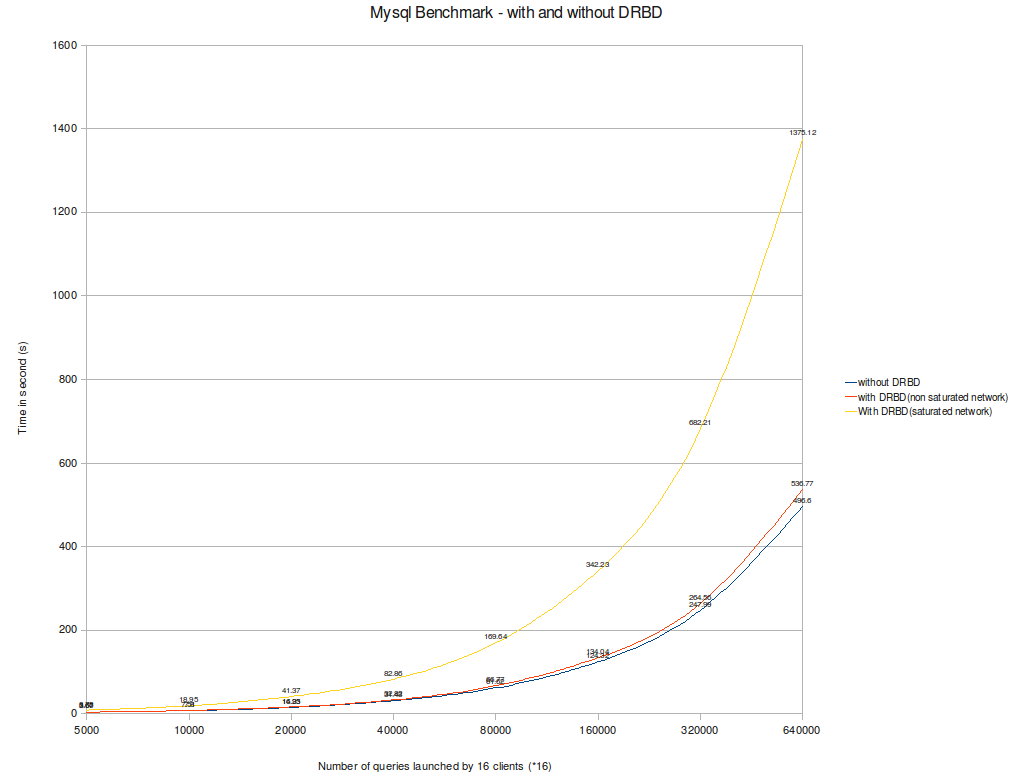
\includegraphics[scale=0.5]{schema/drbd-test.png}
\end{center}
\caption{DRBD benchmark} 
\label{hb-gui-2nodes} 
\end{figure}

You can see that DRBD offer good performance in general. It can be use on OAR without hesitation.



\section{Global system test on Debian}
\subsection{2 nodes - Postgres}
\begin{itemize}
 \item Migrate resources by set nodes in standby mode : Test OK, heartbeat launches resources on the backup, and when the primary come back, resources are migrate on the primary.
 \item Power off/power on the master server (with IPMI, kareboot) : Test OK, resources migrate after a time, about 60s, which correspond at cluster delay. When the master node is anew alive, resources migrate on the master node.
 \item Power off/power on the backup server (with IPMI, kareboot), without resources : Test OK, the server is down. Heartbeat let its resources on the master.
 \item \textit{Killall -9 Almighty} on primary : Test OK, the master relaunch oar-server.
 \item \textit{killall -9 postgres} : Test OK, the master stop oar-server, launch postgres and after oar-server.
 \item \textit{Killall -9 Almighty} and comment the line in /etc/init.d/oar-server for start the daemon : Test OK, heartbeat don't arrive to restart oar-server, so it migrate resources on the backup.
But after uncomment the line on master, you must cleanup resource otherwise heartbeat don't want restart resource. See \ref{hb-command}.
 \item Add rule in iptable for drop all communications : heartbeat and DRBD (iptables -A OUTPUT -p tcp --dport 7788 -j DROP, ...). Heartbeat launch resources on the two nodes. DRBD are primary on the two nodes and work with standalone mode. When the network come bask, heartbeat launch resources on the master, but DRBD stay in standalone mode. It is the problem of split brain. It can be solve manually (See \ref{drbd-admn}).
Admin can enter his mail in the drbd split brain handler for know when drbd is in standalone mode. Test OK, but heartbeat need admin intervention.
 \item Heartbeat, in my configuration, have two links. The test now is two disconnect one of the two links : Test OK, heartbeat continue to run. In the log (\textit{/var/log/ha-log}), you can see Link node eth1 dead.
\end{itemize}

\textbf{Software test} : 2 servers (with postgres), 1 frontend, 1 node (resource). All commands are typed from the frontend.
\begin{itemize}
 \item execute \textit{oarnodes}, standby the master, and retry oarnodes : Test OK
 \item Reserve resource (oarsub -I), and after first node connection, standby the server, and disconnect, WITHOUT detach : Test failed, the job is not ended, and stay alive.
 \item Reserve resource (oarsub -I), and after first node connection, standby the server, and disconnect, WITH detach : Test OK ! The job continue to run, and when the user quit, the new oar-server arrives to kill the job, properly !
If the job is ended before the backup is up, the job is not deleted immediately, but after a few time. In the job events, we  can see : SWITCH\_INTO\_TERMINATE\_STATE:[bipbip 4] Ask to change the job state. After that, the job is killed.
In oarexec code, function quit\_oarexec : loop until the daemon has inform server.
 \item Reserve resource (oarsub -I), reserve a new resource again. The second user wait because there is just one resource. Standby the server. The first job continue to run, the second always waiting. When the first job is ended, the second job begin ! It's very interesting, the job start it's scheduling on the master oar server, and is authorized  by the backup oar server.
 \item Execute oarstat, standby the master node, and execute oarstat : Test OK
\end{itemize}


\subsection{2 nodes - Mysql}

\begin{itemize}
 \item Migrate resources by set nodes in standby mode : Test OK, heartbeat launches resources on the backup, and when the primary come back, resources are migrate on the primary.
 \item Power off/power on the master server (with IPMI, kareboot) : Test OK.
 \item Power off/power on the backup server (with IPMI, kareboot), without resources : Test OK.
 \item \textit{Killall -9 Almighty} on primary : Test OK.
 \item \textit{/etc/init.d/mysql stop} : Test OK.
 \item \textit{Killall -9 Almighty} and comment the line in /etc/init.d/oar-server for start the daemon : Test OK, but admin have to cleanup resource before it can't be migrate on the failed node. See \ref{hb-command}.
 \item Add rule in iptable for drop all communications : heartbeat and DRBD (iptables -A OUTPUT -p tcp --dport 7788 -j DROP, ...). Heartbeat launch resources on the two nodes. DRBD are primary on the two nodes and work with standalone mode. When the network come bask, heartbeat launch resources on the master, but DRBD stay in standalone mode. It is the problem of split brain. It can be solve manually (See \ref{drbd-admn}).
Admin can enter his mail in the drbd split brain handler for know when drbd is in standalone mode. Test OK, but heartbeat need admin intervention.
 \item Heartbeat, in my configuration, have two links. The test now is two disconnect one of the two links : Test OK, heartbeat continue to run. In the log (\textit{/var/log/ha-log}), you can see Link node eth1 dead.
\end{itemize}

\textbf{Software test} : 2 servers (with mysql), 1 frontend, 1 node (resource). All commands are typed from the frontend.
\begin{itemize}
 \item execute \textit{oarnodes}, standby the master, and retry oarnodes : Test OK, oarnodes say : try to connect... until the backup is alive.
 \item Reserve resource (oarsub -I), and after first node connection, standby the server, and disconnect, WITHOUT detach : Test failed, the job is still running...
 \item Reserve resource (oarsub -I), and after first node connection, standby the server, and disconnect, WITH detach : Test OK ! The job continue to run, and when the user quit, the new oar-server arrives to kill the job, properly !
If the job is ended before the backup is up, the job is not deleted immediately, but after a few time. In the job events, we  can see : SWITCH\_INTO\_TERMINATE\_STATE:[bipbip 4] Ask to change the job state. After that, the job is killed.
In oarexec code, function quit\_oarexec : loop until the daemon has inform server.
 \item Reserve resource (oarsub -I), reserve a new resource again. The second user wait because there is just one resource. Standby the server. The first job continue to run, the second always waiting. When the first job is ended, the second job begin ! It's very interesting, the job start it's scheduling on the master oar server, and is authorized  by the backup oar server.
 \item Execute oarstat, standby the master node, and execute oarstat : Test OK, the commands work, it print the same results. If we launch the command during the fail-over, the command inform users that it can't connect to the database, wait few seconds...
\end{itemize}


\subsection{4 nodes - Postgres}
\begin{itemize}
 \item Migration test (master oar-server) : Test OK
 \item Migration test (master Postgres) : Test OK
 \item Power off/power on the master postgres server (IPMI kareboot) : Test OK, migration after a timer
 \item Power off/power on the master oar server (IPMI kareboot) : Test OK
 \item Power off/power on the backup oar server (IPMI kareboot), with resources : Test OK
 \item Power off/power on the backup postgres server (IPMI kareboot), without resources : Test OK
 \item \textit{killall -9 Almighty} on oar-server : Test OK
 \item \textit{killall -9 postgres} : Test OK
\end{itemize}

\textbf{Software test} : 4 servers (with postgres), 1 frontend, 1 node (resource). All commands are typed from the frontend.
\begin{itemize}
 \item execute oarnodes, standby the oar master, and retry oarnodes : Test OK
 \item execute oarnodes, standby the postgresql master, and retry oarnodes : Test OK
 \item execute oarstat, standby the oar master, and retry oarnodes : Test OK
 \item execute oarstat, standby the postgres master, and retry oarnodes : Test OK
 \item Reserve resource (oarsub -I), and after first node connection, standby the oar-server, and disconnect, WITHOUT detach : Test failed. The job is not ended.
 \item Reserve resource (oarsub -I), and after first node connection, standby the oar-server, and disconnect, WITH detach : Test OK, the job is deleted when the user exit.
 \item Reserve resource (oarsub -I), and after first node connection, standby the postgres server, and disconnect, WITH detach : Test OK, the job is deleted when the user exit.
 \item Reserve resource (oarsub -I), reserve a new resource again. The second user wait because there is just one resource. Standby the oar-server. The first job continue to run, the second always waiting. When the first job is ended, the second job begin ! It's very interesting, the job start it's scheduling on the master oar server, and is authorized  by the backup oar server. Test OK.
\end{itemize}


\subsection{4 nodes - Mysql}

\begin{itemize}
 \item Migration test (master oar-server) : Test OK
 \item Migration test (master Mysql) : Test OK
 \item Power off/power on the master oar server (IPMI kareboot) : Test OK. After node reboot, resources returns on the master.
 \item Power off/power on the master mysql server (IPMI kareboot) : Test OK.
 \item Power off/power on both master mysql and oar server (IPMI kareboot) : Test OK. Don't forget to disable quorum policy !
 \item Power off/power on both master mysql and oar server + backup DB (IPMI kareboot) : Test OK, oar services continue to run to backup. the database is launched when the first DB node come back.
 \item Power off/power on backup mysql (IPMI kareboot) : Test OK. After node reboot, standby the primary to check if everything is OK.
 \item Power off/power on 4 nodes : Test OK.
 \item \textit{killall -9 Almighty} on oar-server : Test OK, resources is relaunched on the same server.
 \item \textit{killall -9 mysqld} : Test OK
 \item \textit{killall -9 mysqld} + unmount mysql partition (/mnt/drbddata) : Test OK, heartbeat detect filesystem error, relaunch it, and restart mysql.
 \item \textit{drbdadmn disconnect all} : Test failed, heartbeat don't detect problems.
\end{itemize}

\textbf{Software test} : 4 servers (with mysql), 1 frontend, 1 node (resource). All commands are typed from the frontend.\\
Same results as Postgres with 4 nodes configurations.


















\appendix
\chapter{DRBD example configuration}
\label{drbdexample}
\begin{lstlisting}
global { usage-count no; }
resource mysql {
	protocol C;
	startup {
		wfc-timeout 120;
	}
	disk {
		on-io-error detach;
	}
	syncer {
		rate 700000K;
		al-extents 257;
	}
	on node1{
		device DRBDPARTITION;
		disk DISKPARTITION;
		address node2:DBRDPORT;
		meta-disk internal;
	}
	on node2{
		device DRBDPARTITION;
		disk DISKPARTITION;
		address node1:DBRDPORT;
		meta-disk internal;
	}
	net {
		after-sb-0pri discard-younger-primary;
		after-sb-1pri consensus;
 		after-sb-2pri call-pri-lost-after-sb;
	}
	handlers {
		split-brain "echo Splitbraindetected >> /var/log/drbd-log";
		pri-lost-after-sb "echo pri-lost-after-sb >> /var/log/drbd-log";
	}
}
\end{lstlisting}





\chapter{Heartbeat example configuration on Debian}
\label{cibexample}
\section {High Availability on OAR with 2 nodes configuration, postgresql database}
\begin{lstlisting}[language=xml]

<cib admin_epoch="0" have_quorum="true" ignore_dtd="false" num_peers="1" cib_feature_revision="2.0" generated="false" epoch="4" num_updates="4" cib-last-written="Mon Jul 20 15:22:44 2009" ccm_transition="1">
   <configuration>
   
   
     <crm_config>
       <cluster_property_set id="cib-bootstrap-options">
	 <attributes>
	   <nvpair id="cib-bootstrap-options-symmetric-cluster" name="symmetric-cluster" value="true"/>
	   <nvpair id="cib-bootstrap-options-no-quorum-policy" name="no-quorum-policy" value="stop"/>
	   <nvpair id="cib-bootstrap-options-default-resource-stickiness" name="default-resource-stickiness" value="0"/>
	   <nvpair id="cib-bootstrap-options-default-resource-failure-stickiness" name="default-resource-failure-stickiness" value="0"/>
	   <nvpair id="cib-bootstrap-options-stonith-enabled" name="stonith-enabled" value="false"/>
	   <nvpair id="cib-bootstrap-options-stonith-action" name="stonith-action" value="reboot"/>
	   <nvpair id="cib-bootstrap-options-startup-fencing" name="startup-fencing" value="true"/>
	   <nvpair id="cib-bootstrap-options-stop-orphan-resources" name="stop-orphan-resources" value="true"/>
	   <nvpair id="cib-bootstrap-options-stop-orphan-actions" name="stop-orphan-actions" value="true"/>
	   <nvpair id="cib-bootstrap-options-remove-after-stop" name="remove-after-stop" value="false"/>
	   <nvpair id="cib-bootstrap-options-short-resource-names" name="short-resource-names" value="true"/>
	   <nvpair id="cib-bootstrap-options-transition-idle-timeout" name="transition-idle-timeout" value="5min"/>
	   <nvpair id="cib-bootstrap-options-default-action-timeout" name="default-action-timeout" value="20s"/>
	   <nvpair id="cib-bootstrap-options-is-managed-default" name="is-managed-default" value="true"/>
	   <nvpair id="cib-bootstrap-options-cluster-delay" name="cluster-delay" value="60s"/>
	   <nvpair id="cib-bootstrap-options-pe-error-series-max" name="pe-error-series-max" value="-1"/>
	   <nvpair id="cib-bootstrap-options-pe-warn-series-max" name="pe-warn-series-max" value="-1"/>
	   <nvpair id="cib-bootstrap-options-pe-input-series-max" name="pe-input-series-max" value="-1"/>
	   <nvpair id="cib-bootstrap-options-dc-version" name="dc-version" value="2.1.3-node: 552305612591183b1628baa5bc6e903e0f1e26a3"/>
	 </attributes>
       </cluster_property_set>
     </crm_config>
     
     
     
     
     <resources>
       <group id="group_1">
	 <primitive class="ocf" id="VirtualIP" provider="heartbeat" type="IPaddr2">
	   <operations>
	     <op id="VirtualIP_mon" interval="5s" name="monitor" timeout="5s"/>
	   </operations>
	   <instance_attributes id="VirtualIP_inst_attr">
	     <attributes>
	       <nvpair id="VirtualIP_attr_0" name="ip" value="172.16.16.220"/>
	       <nvpair id="VirtualIP_attr_1" name="nic" value="eth1"/>
	       <nvpair id="VirtualIP_attr_2" name="cidr_netmask" value="24"/>
	     </attributes>
	   </instance_attributes>
	 </primitive>
	 <primitive class="heartbeat" id="DRBD-disk" provider="heartbeat" type="drbddisk">
	   <operations>
	     <op id="DRBD-disk_mon" interval="120s" name="monitor" timeout="60s"/>
	   </operations>
	   <instance_attributes id="DRBD-diskinst_attr">
	     <attributes>
	       <nvpair id="DRBD-disk_attr_1" name="1" value="mysql"/>
	     </attributes>
	   </instance_attributes>
	 </primitive>
	 <primitive class="ocf" id="Filesystem" provider="heartbeat" type="Filesystem">
	   <operations>
	     <op id="Filesystem_mon" interval="120s" name="monitor" timeout="60s"/>
	   </operations>
	   <instance_attributes id="Filesystem_inst_attr">
	     <attributes>
	       <nvpair id="Filesystem_attr_0" name="device" value="/dev/drbd0"/>
	       <nvpair id="Filesystem_attr_1" name="directory" value="/mnt/drbddata"/>
	       <nvpair id="Filesystem_attr_2" name="fstype" value="ext3"/>
	     </attributes>
	   </instance_attributes>
	 </primitive>
	 <primitive id="Postgres" class="lsb" type="postgresql-8.3" provider="heartbeat">
	   <operations>
	     <op id="Postgres_mon" interval="120s" name="monitor" timeout="60s"/>
	   </operations>
	   <meta_attributes id="Postgres_meta_attrs">
	     <attributes>
	       <nvpair id="Postgres_metaattr_target_role" name="target_role" value="started"/>
	     </attributes>
	   </meta_attributes>
	 </primitive>
	 <primitive class="lsb" id="oar-server" provider="heartbeat" type="oar-server">
	   <operations>
	     <op id="oar-server_mon" interval="120s" name="monitor" timeout="60s"/>
	   </operations>
	 </primitive>
	 <meta_attributes id="group_1_meta_attrs">
	   <attributes>
	     <nvpair id="group_1_metaattr_ordered" name="ordered" value="true"/>
	   </attributes>
	 </meta_attributes>
       </group>
     </resources>
     
     
     
     
     <constraints>
       <rsc_location id="rsc_location_group_1" rsc="group_1">
	 <rule id="prefered_location_group_1" score="100">
	   <expression attribute="#uname" id="prefered_location_group_1_expr" operation="eq" value="node1"/>
	 </rule>
       </rsc_location>
     </constraints>
     
     
   </configuration>
 </cib>
\end{lstlisting}


\section {High Availability on OAR with 4 nodes configuration}
\begin{lstlisting}[language=xml]
<cib generated="false" admin_epoch="0" have_quorum="false" ignore_dtd="false" num_peers="1" cib_feature_revision="2.0" epoch="72" num_updates="1" cib-last-written="Wed Jul 22 13:16:03 2009" ccm_transition="1">
   <configuration>


     <crm_config>
       <cluster_property_set id="cib-bootstrap-options">
         <attributes>
           <nvpair id="cib-bootstrap-options-dc-version" name="dc-version" value="2.1.3-node: 552305612591183b1628baa5bc6e903e0f1e26a3"/>
           <nvpair id="cib-bootstrap-options-symmetric-cluster" name="symmetric-cluster" value="false"/>
           <nvpair id="cib-bootstrap-options-no-quorum-policy" name="no-quorum-policy" value="ignore"/>
           <nvpair id="cib-bootstrap-options-default-resource-stickiness" name="default-resource-stickiness" value="0"/>
           <nvpair id="cib-bootstrap-options-default-resource-failure-stickiness" name="default-resource-failure-stickiness" value="0"/>
           <nvpair id="cib-bootstrap-options-stonith-enabled" name="stonith-enabled" value="false"/>
           <nvpair id="cib-bootstrap-options-stonith-action" name="stonith-action" value="reboot"/>
           <nvpair id="cib-bootstrap-options-startup-fencing" name="startup-fencing" value="true"/>
           <nvpair id="cib-bootstrap-options-stop-orphan-resources" name="stop-orphan-resources" value="true"/>
           <nvpair id="cib-bootstrap-options-stop-orphan-actions" name="stop-orphan-actions" value="true"/>
           <nvpair id="cib-bootstrap-options-remove-after-stop" name="remove-after-stop" value="false"/>
           <nvpair id="cib-bootstrap-options-short-resource-names" name="short-resource-names" value="true"/>
           <nvpair id="cib-bootstrap-options-transition-idle-timeout" name="transition-idle-timeout" value="5min"/>
           <nvpair id="cib-bootstrap-options-default-action-timeout" name="default-action-timeout" value="20s"/>
           <nvpair id="cib-bootstrap-options-is-managed-default" name="is-managed-default" value="true"/>
           <nvpair id="cib-bootstrap-options-cluster-delay" name="cluster-delay" value="60s"/>
           <nvpair id="cib-bootstrap-options-pe-error-series-max" name="pe-error-series-max" value="-1"/>
           <nvpair id="cib-bootstrap-options-pe-warn-series-max" name="pe-warn-series-max" value="-1"/>
           <nvpair id="cib-bootstrap-options-pe-input-series-max" name="pe-input-series-max" value="-1"/>
         </attributes>
       </cluster_property_set>
     </crm_config>




     <resources>
       <group id="Database-servers">
         <meta_attributes id="Database-servers_meta_attrs">
           <attributes>
             <nvpair name="target_role" id="Database-servers_metaattr_target_role" value="started"/>
             <nvpair id="Database-servers_metaattr_ordered" name="ordered" value="true"/>
             <nvpair id="Database-servers_metaattr_collocated" name="collocated" value="true"/>
           </attributes>
         </meta_attributes>
         <primitive class="ocf" type="IPaddr2" provider="heartbeat" id="VirtualIP-database">
           <operations>
             <op id="IPaddr2_mon" interval="5s" name="monitor" timeout="5s"/>
           </operations>
           <instance_attributes id="VirtualIP-database_instance_attrs">
             <attributes>
               <nvpair id="89b87cae-b271-4d55-8881-c89508ad8451" name="ip" value="172.16.16.221"/>
               <nvpair id="bff53b6b-a11d-4cb0-8db3-24ef1b82fbb0" name="nic" value="eth1"/>
               <nvpair id="d6dc4cd1-b057-48be-91c7-3b733e066269" name="cidr_netmask" value="24"/>
             </attributes>
           </instance_attributes>
           <meta_attributes id="VirtualIP-database_meta_attrs">
             <attributes>
               <nvpair name="target_role" id="VirtualIP-database_metaattr_target_role" value="started"/>
             </attributes>
           </meta_attributes>
         </primitive>
         <primitive id="DRBD-disk" class="heartbeat" type="drbddisk" provider="heartbeat">
           <operations>
             <op id="DRBD-disk_mon" interval="120s" name="monitor" timeout="60s"/>
           </operations>
           <instance_attributes id="DRBD-disk_inst_attr">
             <attributes>
               <nvpair id="DRBD-disk_attr_1" name="1" value="mysql"/>
             </attributes>
           </instance_attributes>
           <meta_attributes id="DRBD-disk_meta_attrs">
             <attributes>
               <nvpair id="DRBD-disk_metaattr_target_role" name="target_role" value="started"/>
             </attributes>
           </meta_attributes>
         </primitive>
         <primitive id="Filesystem" class="ocf" type="Filesystem" provider="heartbeat">
           <operations>
             <op id="Filesystem_mon" interval="120s" name="monitor" timeout="60s"/>
           </operations>
           <instance_attributes id="Filesystem_instance_attrs">
             <attributes>
               <nvpair id="29b7a79c-ad8f-47ef-91dd-610292acac10" name="device" value="/dev/drbd0"/>
               <nvpair id="639a3cc9-8df6-497a-b874-f04b72da5577" name="directory" value="/mnt/drbddata"/>
               <nvpair id="1e59d136-4bc7-4f6c-9eb4-a62e06ec48d1" name="fstype" value="ext3"/>
             </attributes>
           </instance_attributes>
           <meta_attributes id="Filesystem_meta_attrs">
             <attributes>
               <nvpair id="Filesystem_metaattr_target_role" name="target_role" value="started"/>
             </attributes>
           </meta_attributes>
         </primitive>
         <primitive id="MysqlHA" class="lsb" type="mysqlha" provider="heartbeat">
           <operations>
             <op id="MysqlHA_mon" interval="120s" name="monitor" timeout="60s"/>
           </operations>
           <meta_attributes id="MysqlHA_meta_attrs">
             <attributes>
               <nvpair id="MysqlHA_metaattr_target_role" name="target_role" value="started"/>
             </attributes>
           </meta_attributes>
         </primitive>
       </group>
       <group id="OAR-servers">
         <meta_attributes id="OAR-servers_meta_attrs">
           <attributes>
             <nvpair id="OAR-servers_metaattr_target_role" name="target_role" value="stopped"/>
             <nvpair id="OAR-servers_metaattr_ordered" name="ordered" value="true"/>
             <nvpair id="OAR-servers_metaattr_collocated" name="collocated" value="true"/>
           </attributes>
         </meta_attributes>
         <primitive id="VirtualIP-OAR-server" class="ocf" type="IPaddr2" provider="heartbeat">
           <operations>
             <op id="VirtualIP-OAR-server_mon" interval="5s" name="monitor" timeout="5s"/>
           </operations>
           <instance_attributes id="VirtualIP-OAR-server_instance_attrs">
             <attributes>
               <nvpair id="bb615f47-387e-46cb-945f-8757d494791b" name="ip" value="172.16.16.220"/>
               <nvpair id="6fe16a0e-c414-4a5b-8e5f-f0c48b369770" name="nic" value="eth1"/>
               <nvpair id="b25acc28-5186-4a22-9433-5347017cdc71" name="cidr_netmask" value="24"/>
             </attributes>
           </instance_attributes>
           <meta_attributes id="VirtualIP-OAR-server_meta_attrs">
             <attributes>
               <nvpair id="VirtualIP-OAR-server_metaattr_target_role" name="target_role" value="started"/>
             </attributes>
           </meta_attributes>
         </primitive>
         <primitive id="OAR-server" class="lsb" type="oar-server" provider="heartbeat">
           <operations>
             <op id="OAR-server_mon" interval="120s" name="monitor" timeout="60s"/>
           </operations>
           <meta_attributes id="OAR-server_meta_attrs">
             <attributes>
               <nvpair id="OAR-server_metaattr_target_role" name="target_role" value="started"/>
             </attributes>
           </meta_attributes>
         </primitive>
       </group>
     </resources>




     <constraints>
       <rsc_location id="location-Database" rsc="Database-servers">
         <rule id="prefered_location-Database" score="0">
           <expression attribute="#uname" id="f968a0dd-59dd-4d02-b54a-36c7139afa13" operation="ne" value="node1"/>
           <expression attribute="#uname" id="0ef6e38b-6a34-4e23-bc22-9dccfacc95b6" operation="ne" value="node3"/>
         </rule>
       </rsc_location>
       <rsc_location id="location-OAR" rsc="OAR-servers">
         <rule id="prefered_location-OAR" score="0">
           <expression attribute="#uname" id="4d2c21d8-aea7-460b-bfeb-cd6d22e4a17e" operation="ne" value="node2"/>
           <expression attribute="#uname" id="3292b1b4-04cb-4650-b6e0-2e4428c837a8" operation="ne" value="node4"/>
         </rule>
       </rsc_location>
       <rsc_location id="location_Master-OAR" rsc="OAR-servers">
         <rule id="prefered_location_Master-OAR" score="INFINITY">
           <expression attribute="#uname" id="37a60f84-c7ed-4e4a-835a-55382961c990" operation="eq" value="node1"/>
         </rule>
       </rsc_location>
       <rsc_location id="location_Master-Database" rsc="Database-servers">
         <rule id="prefered_location_Master-Database" score="INFINITY">
           <expression attribute="#uname" id="37a78f84-c7ed-4e4a-835a-54382451c990" operation="eq" value="node2"/>
         </rule>
       </rsc_location>
     </constraints>


   </configuration>
 </cib>
\end{lstlisting}

\end{document}          
